%%%%%%%%%%%%%%%%%%%%%%%%%%%%%%%%%%%%%%%%%
% EPFL/Blue Brain Project
%
% Author:
% 	Quarta Jonny
%
% Date:
%	June 2014
%
%%%%%%%%%%%%%%%%%%%%%%%%%%%%%%%%%%%%%%%%%

%----------------------------------------------------------------------------------------
%	PACKAGES AND DOCUMENT CONFIGURATIONS
%----------------------------------------------------------------------------------------

\documentclass{article}


\usepackage{graphicx} % Required for the inclusion of images
\usepackage{multicol}



\setlength\parindent{0pt} % Removes all indentation from paragraphs

\renewcommand{\labelenumi}{\alph{enumi}.} % Make numbering in the enumerate environment by letter rather than number (e.g. section 6)


%----------------------------------------------------------------------------------------
%	DOCUMENT INFORMATION
%----------------------------------------------------------------------------------------

\title{\textbf{Reinforcement Learning techniques \\ for ball controlling using the SpiNNaker}} % Title

\author{Jonny \textsc{Quarta}} % Author name

%\date{\today} % Date for the report

\begin{document}

\maketitle % Insert the title, author and date

\tableofcontents

%----------------------------------------------------------------------------------------
%	SECTION 1
%----------------------------------------------------------------------------------------

\section{Project Overview}
During the last decades, machine learning and control theory underwent astonishing advances. New algorithms are continously created and optimization techniques are invented with the purpose to speed up the systems. Such methods are however almost always sequential and parallelization is rarely applied in order to speed up event more the systems. \\

The aim of this project is that on a first step reinforcement learning techniques are used on a simple control problem. Then, parallelization strategies are adopted in order to speed up the sequential solution and the two systems are then compared. \\ \\

The idea is to control a ball hanging on a plate and equilibrate it toward the plate center, using neural networks coupled to basic reinforcement learning rules. The plate is controlled by two motors, which can apply different inclination angles so that the plate can be inclined in many ways. Therefore, two degrees of freedom determine the plate state. A camera is situated above the plate and its purpose is to detect the ball position and send it to the control system, which will then compute the next plate inclination.\\

The hardware responsible for all computations is the SpiNNaker, a neuromorphic device designed at the University of Manchester. The version we use is composed of 4 chips, each of them containing 16 cores.\\
This hardware enables the user to simulate a single or a population of neurons on each core, highly distributing the computation. The final purpose is to mimic as much as possible the very highly parallel brain structure. \\

By using this structure, it is possible to build very efficient applications running almost in real-time (compared to a sequential implementation). This is exactly what we want, because in order to balance the ball, once the position is recorded, it is really important to compute the new motor angles as fast as possible, otherwise the algorithm would never converge (or would converge slowly). \\ \\

The next two sections will describe the theory behing ball control. Then, the SpiNNaker architecture and other hardware components are presented and the actual implementation detailed. On a next step, parallelization strategies are showed and finally results are provided.


\section{Control System Theory}
During this section, the theory behind reinforcement learning techniques (later used in the project) is presented.\\

In order to control the ball in a consistent manner, we first need to track its position and transform this information so that the control system can understant it.
The idea is to virtually sample the plate into different areas, each of them corresponding to the \textbf{receptive field} of a neuron (or a population, as we finally will use \textbf{Mean-Field Populations}). These neurons are connected to a main node, constructing therefore a neural network having a Perceptron structure. The main concept changing from a normal Perceptron is that the updating rules (based on reinforcement learning) are different and particular feature vectors representing each neuron are added. \\ \\

The control system is split into two major components: the \textbf{Actor} and the \textbf{Critic} systems. The first one is responsible for controlling the motor output, whereas the latter is responsible for evaluating a \textbf{value function} used to converge toward a ball stabilization position (in this case the plate center). Each one of them is actually composed of a neural network with different parameters which will be updated at each algorithm iteration. \\ \\

Now, the control theory will be described. \\
The first important concept in reinforcement learning is the \textbf{reward}, which represents the final goal of the system. In this case, we want the ball to be situated at the plate center. If the ball is situated on that position, the reward would be 1, otherwise the farther the ball is located, the more the reward decrases (0 is the lower limit). In addition, we also take into account ball speed. The final purpose is that the position is in the center, but also that there is no speed. \\ \\

Therefore, the reward R(x) is calculated as follows:
\[
R(x) = r(x) - s(\dot{\theta})
\]
where r(x) is the component based on the ball position, whereas \(s(\dot{\theta})\) determines the ball speed component. Finally,
\[
r(x) = 1 - x
\]
and
\[
s(\theta) = \theta
\]
In order to keep the latter component less important than the position, the speed as been rescaled by a factor of \(\frac{1}{10}\), so that its maximum value never reaches more than 0.3. In this extreme case, s(\(\theta\)) has a maximum value of 0.3, implying that R(x) lies in a range of [-0.3;1].


\section{Parameters Updating}

\subsection{Critic System Updating}
In order to check for the goal achievement, we need to verify if the real reward (the ball on the center) is very close to the cumulative expected reward, calculated from the Critic neural network. Then, we can define the error:
\[
\delta(t) = R(t) + \frac{1}{\Delta t}((1 - \frac{\Delta t}{\tau})V(t) - V(t - \Delta t))
\]
where \(V(t)=V(x(t), w^{V})\) is the expected value after a certain time (in this case computed by the Critic neural network). Note that as the algorithm progresses, V(t) converges to the same value of R(t), which is 1, decreasing the total error.\\
We can also rewrite the last statement in a more simple way:
\[
\delta(t) = R(t) + \gamma V(t) - V(t - \Delta t)
\]
where
\[
\gamma = 1 - \frac{\Delta t}{\tau}
\]

The last part involves the parameters updating. This is accomplished with the concept of \textbf{eligibility trace}. The basic updating rules are:
\[
\Delta e_{i}(t) = -\frac{1}{\kappa}e_{i}(t) + \frac{\delta V(x(t), w^{V})}{\delta w_{i}^{V}}, 0 < \kappa <= \tau
\]
\[
\Delta w_{i}^{V} = \eta^{V} \delta (t)e_{i}(t)
\]
where \(\eta^{V}\) is the Critic network learning rate. \\ \\

In order to update \(e_{i}(t)\), we must discretize it (solve it numerically). The way to do is:
\[
e_{i}(t + \Delta t) = \lambda \gamma e_{i}(t) + \frac{\delta V(x(t), w^{V})}{\delta w_{i}^{V}}
\]
with
\[
\lambda = \frac{1 - \frac{\Delta t}{\kappa}}{1 - \frac{\Delta t}{\tau}}
\]


\subsection{Actor System Updating}
The last part involves the Actor network updating. It must take the final decision about the motor commands and the way this is achieved is by using the function
\[
u(t) = s(A(x(t), w^{A})) + \sigma n(t))
\]
where A is the Actor neural network, n(t) the noise and s(x) a special function determining the actual motor commands. The factor \(\sigma\), used for rescaling the noise, is defined by
\[
\sigma = \sigma_{0} min(k, max(0, 1 - V(t)))
\]
so that as the value (V(t)) approaches 1, the rescaling factor becomes less and less important (and vice-versa, if the value is 0, the noise is very important). On the other hand, the real noise is implemented using Box-Muller transformation in order to obtain a 0 mean, 1 variance gaussian noise. Note that noise is used in order to implement exploratory moves. \\ \\


Finally, in order to achieve the goal, the Actor neural network weights must be updated (using some sort of gradient descent):  
\[
\Delta w_{i}^{A} = \eta^{A}\delta (t)n(t)\frac{\delta A(x(t), w^{A})}{\delta w_{i}^{A}}
\]
where \(\eta^{A}\) is the Actor network learning rate. As the error \(\delta\) decreases, we update the weights less and less. \\



\section{Neural Networks Structure}
As previously exposed, the control system contains 2 neural networks: the actor A and the critic V.

\subsection{Critic Neural Network Structure}
The critic neural network is responsible for determining the expected values. Its structure corresponds to the Perceptron:
\[
V(x) = \frac{1}{N^{V}} \sum_{i=1}^{N^{V}}{w_{i}^{V}\phi_{i}^{V}(x)}
\]
where \(w_{i}^{V}\) are the weights. Note that \(\phi_{i}^{V}(x)\) is a feature vector, which will represent the space (into the plate) discretization of the neural network. Here, each neuron has a receptive field defined by a center and a distance measure. The distance measure from the center to the ball position decide the neuron firing rate.\\
The exact meaning of the feature vector will be discussed in the next section.

The last important part is the gradient computation used during the update, which is simply given by:
\[
\frac{\delta V(x(t), w^{V})}{\delta w_{k}^{V}} = \frac{\delta \sum_{i=1}^{N^{V}}{w_{i}^{V}\phi_{i}^{V}(x)}}{\delta w_{k}^{V}} = \phi_{k}^{V}
\]
\\
In practice, for optimization reasons, the Critic system has been split into two neural networks, each one along a different axis:
\[
V_{x}(p) = \frac{1}{N^{V}} \sum_{i=1}^{N^{V}}{w_{x,i}^{V}\phi_{x,i}^{V}(p)}
\]
and
\[
V_{y}(p) = \frac{1}{N^{V}} \sum_{i=1}^{N^{V}}{w_{y,i}^{V}\phi_{y,i}^{V}(p)}
\]
Note that here p defines the ball position vector. The feature vectors measure the distance from the neuron center to the ball position along the different axis. Finally, all update rules apply independently on each axis.


\subsection{Actor Neural Network Structure}
The actor neural network is responsible for determining the system output. Its structure corresponds to the Perceptron as well:
\[
A(x) = \frac{1}{N^{A}} \sum_{i=1}^{N^{A}}{w_{i}^{A}\phi_{i}^{A}(x)}
\]
where \(w_{i}^{A}\) the weights. Note that \(\phi_{i}^{A}(x)\) is a feature vector that has to be determined, indicating that the input (e.g. ball position) must be somehow transformed before being introduced into the network. \\
In practice, this network must output two angles, \(\theta\) and \(\psi\), which are coupled to the axis of the Critic network, and is therefore defined by two neural networks:
\[
\theta (x) = \frac{1}{N^{A}} \sum_{i=1}^{N^{A}}{w_{\theta, i}^{A}\phi_{x,i}^{A}(x)}
\]

\[
\psi (x) = \frac{1}{N^{A}} \sum_{i=1}^{N^{A}}{w_{\psi, i}^{A}\phi_{y,i}^{A}(x)}
\]

The feature vectors are the same as in the Critic neural network. Therefore, they are also discretized in space.\\
The space discretization will be deeper discussed in the next sections. Finally, as for the Critic network, all update rules apply independently on each angle.


\section{Mean-Field Populations}

\subsection{Basic Notions}
When dealing with neural networks, usually huge quantities of neurons have to be simulated. This can be very power consuming and slow. Of course, as the hardware power grows, more neurons can be simulated in a decent time. A way to partially solve this problem is to reduce an entire neural population to a single unit by averaging all the parameters and activity. This decreases the simulation complexity by approximating quite well the actual network behaviour. \\

Let assume we have a neuronal model (the Tsodyks-Markram model) defined by the following equations:
\[
\frac{dx}{dt} = \frac{z}{\tau_{rec}} - U_{SE}\: x\: \delta (t - t_{sp})
\]

\[
\frac{dy}{dt} = -\frac{y}{\tau_{in}} + U_{SE}\: x\: \delta (t - t_{sp})
\]

\[
\frac{dz}{dt} = \frac{y}{\tau_{in}} - \frac{z}{\tau_{rec}}
\]

\[
\frac{d U_{SE}}{dt} = -\frac{U_{SE}}{\tau_{fac}} + U_{SE}^{0}(1 - U_{SE})\delta(t - t_{sp})
\]
where there exists some sort of available spike resources important for spike generation. There are three possible states: x (recovered), y (active) and z (inactive). After a pre-synaptic spike, the resources go from the state x to 
y, therefore activating them for generating the post-synaptic spike. After this process, the resources go from y to z, the inactive state, thus not being usable. After a while, they go from z to x, hence becoming available again.\\

\(U_{SE}\) is the resources fraction consumed after every spike, \(t_{sp}\) the time of spike occurring and \(\tau_{rec}, \tau_{fac}, \tau_{in} \) are the resources recovery, synaptic facilitation and inactivation time constants, respectively. Note that \(U_{SE}\) is not constant, thus enabling synaptic facilitation and depletion. Finally, \(U_{SE}^{0}\) determines the increase of \(U_{SE}\) due to spike generation. \\

Assume a population modelled by these equations is created. A Mean-Field characterization of this population is given by:
\[
\tau_{m} \frac{dF_{i}}{dt} = -F_{i} + h(\sum_{J}{J_{i,j} y_{i,j} + I_{i}^{ext}})
\]
where \(\tau_{m}\) is the membrane time constant, \(F_{i}\) the firing rate of population i, \(I_{i}^{ext}\) the external input and \(J_{i,j}\) the weight of the connexion from population j to population i. h is an activation function that has to be determined. Finally, as y can be averaged, we get:
\[
y_{i,j} = \tau_{m} \langle U_{SE}\rangle_{i,j} \: \langle x\rangle_{i,j} \: F_{j} 
\]

\subsection{Applied MFM}
After a very briefly introduction to this field, we come back to the ball control problem. The idea is to apply mean-field populations to the neural networks instead of simulating individual neurons. Note that these transformations apply to both the Actor and Critic neural networks, as they all rely on the same adjacent feature vectors (\(\phi^{V}(x) = \phi^{A}(x) = \phi(x)\)).\\ \\
The basic Perceptron network structure is given by:
\[
P(x) = \sum_{i=1}^{N}{w_{i}\phi_{i}(x)}
\]
As previously explained, the main difference will be \(\phi_{i}\), the feature vector. Instead of characterizing a single neuron, it will represent a mean-field population. Since each population is independent from the others, we can write:
\[
\phi_{i} = F_{i}
\]
where \(F_{i}\) is the population mean firing rate. Then
\[
\frac{dF_{i}}{dt} = \frac{1}{\tau_{m}}(-F_{i} + h(I_{i}^{ext}))
\]
where \(I_{i}^{ext}\) is the external input given by the ball position with respect to the population center. This could be determined by
\[
I_{i}^{ext} = ||\vec{x} - \vec{c}_{i}||
\]
where \(\vec{x}\) is the current ball position and \(\vec{c_{i}}\) the population center. \\
Note that this is in practice slighly modified in order to take into account the axis independence of the system. This function is indeed modified in order to measure the distance along a precice axis:
\[
I_{a,i}^{ext} = abs(\vec{p_{a}} - \vec{c}_{a,i})
\]
where \(a\) can be either x or y (the axis) and \(\vec{p}\) defines the ball position vector.\\

Finally, the activation function is defined by
\[ 
h(I) = \beta(I - \alpha)	\:\: if I >= \alpha, \:0\: otherwise
\]
where \(\beta\) and \(\alpha\) are the slope and the lower threshold, respectively. \\
A very important point is the fact that in order not to connect the populations with each other, their receptive fields must overlap with the ones of their closest neighbours.


\section{System Implementation}
In this section, the actual implementation will be explored.

\subsection{SpiNNaker Architecture}
The SpiNNaker (Spiking Neural Network Architecture) is a multicore computing system whose purpose is to simulate the behaviour of a huge amount of neural populations in real time. The used version contains 4 chips of 16 cpus each, thus a total amount of 64 cores. They communicate by exchanging small packets of about 70 bits, which are entirely handled by the underlying hardware in a very distributed way. This particular design has the purpose of emulating as much as possible the human brain structure.\\

The SpiNNaker also provides an API containing useful functions (accessing core information, performing IO operations, etc..). In the next sections, some of them will be better detailed. A list of the most important ones is situated in the appendix.
\\ \\
The basic loop of the system is:
\begin{verbatim}
void update(uint sim_time, uint none)
{
    if(state == STATE_UNBALANCED) {
        mfm_();
        // actor network updating and command sending
        update_A( sim_time );
        state = move( sim_time );

        // critic networks update
        updateError(x_pos, y_pos, sim_time);
        update_V();
        // end of networks update
    }

    // save step
    if(state != STATE_SAVED && sim_time % SAVE_STEP == 0)           
    {
        save_();
        ... end algorithm
    }
}
\end{verbatim}
This code basically updates the Mean-Field population values as well as the networks parameters and outputs. It also controls the motors. Finally, after a goal state has been reached, the algorithm stops. Note that this function is called every \(\Delta t\) seconds. \\ \\
In the next sub-sections, every step of the algorithm will be detailed.

\subsection{Parameters Initialization}
Before the main loop can be entered, all the network parameters must be initialized. The are mainly two types of parameters that have to be taken into account with care: the network weights and the MFM center positions. \\ \\

When dealing with neural networks, weight initialization is very important and can change the final convergence of the algorithm. In this system, every parameter has been initialized in the following way:
\[
w_{i} = 	\frac{U()}{5} - 0.1; 
\]
where U() randomly generates a number in the range [0;1]. By applying this formula, the weight will have values in the range [-0.1;0.1].\\ \\

The other important parameters are the MFM populations locations. These are initialized in a way so that they take an homogeneous disk shape. As said in the previous 
subsection, cores are arranged in chips. Each chip has a 2D position, as if it were located on a 2D grid. In order to fill the virtual disk, each chip will occupy a circle quarter and each of the 16 cores will be homogeneously placed in this part of the circle. In order to get the chip and core identifiers, the \textit{spin1\_get\_core\_id()} and \textit{spin1\_get\_chip\_id()} functions can be used. The latter returns both the X and Y coordinates in a 32 bits integer, using this format :
\[
[ 0 (16) | Y (8) | X (8) ]
\]
Note that the parenthesis define the number of bits used for a particular field. \\
The homogeneous disk is constructed with the following code:
\begin{verbatim}
int coreX = (coreID & 0x00000003); // 0 to 3
int coreY = (coreID >> 2); // 0 to 3

float p1 = (float)coreX / 4.0;
float p2 = (float)coreY / 4.0;

if(p1 == 0.0) {
	p1 = 0.09;
}

float r = 1.15*sqrt(p1 - 0.05);
float theta = ((PI_/2.0) * p2) + ((PI_/2.0)*(chipX + 2.0*chipY));

float x = r*cos(theta);
float y = r*sin(theta);
\end{verbatim}
Note that the core identifier is used in order to extract two different coordinates. In addition, the \textit{theta} variable is computed by adding a base factor of \( \frac{\Pi }{2}\) multiplied by the chip number. Figure~\ref{fig:disk} shows the results of this processing.

\begin{figure}[h]
\begin{center}
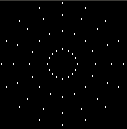
\includegraphics[width=0.3\textwidth]{mfm}
\caption{Homogeneous Disk}
\label{fig:disk}
\end{center}
\end{figure}


\subsection{Position Acquisition}
In order to track the ball, a silicon retina is used. The idea behind this piece of hardware is that instead sending a complete image to the control unit at every frame, the camera does send only detected changes, just like a biological eye. Every received message is a 16 bits integer having the following format:
\[
[ check (1) | X (7) | pol (1) | Y (7) ]
\]
Here, \textit{check} defines a checksum bit, used in order to check for the message consistancy and \textit{pol} defines the polarity of the change (dark to ligh or vice-versa). \\
Once the raw position change is recorded, it cannot be used as such, but has to be processed. The problem is that  the incoming messages correspond to different ball surface points where a change has been detected. Therefore, in order to extract a ball position from this data, we simply average all incoming events within a certain window (in this case of 16 elements).\\
Note that in the system this processing is provided by the \textit{compute\_pos} function, which averages the incoming positions in a very efficient way, without any sum or division. This is accomplished because camera events are very frequent and could be a possible bottleneck.\\

The last step before a position can be usable is the \textbf{normalization}. In order to simplify all the algorithm math, the idea is to approximate the plate by a unit circle, thus having coordinates in a range of [-1;1]. Since the camera send coordinates in a range of [0;128], we can easily use the following transformation (along each axis): 
\[
	x_{norm} = \frac{1}{64}x - 1
\]
In addition, the system also needs the ball speed, which is given by:
\[
	v_{norm} = \frac{x_{norm}(t) - x_{norm}(t - \Delta t)}{\Delta t}
\]
The speed is further divided by a factor of \(\frac{1}{10}\) in order to keep it in a range of [0;0.3]. Fron now on, every position is assumed to be normalized.

\subsection{Motor Output}
In a general way, all the updating rules implemented in the system follow the theory described in the previous sections and therefore are not discussed into further details.\\

The final step is however given by the motor output and is described in this sub-section. \\
The motor system is responsible to move the two motors by a certain angle. The actual values accepted by the system are contained in the range [1500;2500]. Hence, for example, a value of 2000 would define an angle so that the plate is at the default position on that axis (perfectly horizontally). \\
For the reinforcement algorithm purposes, however, such range is not convenient and a [-1;1] would better suit. This is why another normalization is accomplished:
\[
\theta_{norm} = \frac{1}{500}\theta - 4
\]
In this way, in order to place the plate along an axis on a perfectly horizontal position, a value of 0 must be provided.\\ \\

The last important point to consider is the final state of the algorithm. It is indeed important to stop moving the plate as soon as the ball is detected to be located at the center, or better speaking, within a certain range from it. This is why the last part of the output function checks for this condition:
\begin{verbatim}
if(sim_time > 300 && avg_pos < 0.2 && avg_speed < 0.05) {
    sendNormMotorCommand(0.0, 0.0);
    return STATE_BALANCED; // ball balanced
}
else if(sim_time % RESET_STEP == 0) {
    // send an impulse from time to time
    // if the ball is stuck on a place
    if(v_norm(pos_) > 0.7){
        	sendNormMotorCommand(pos_.x, pos_.y);
    }
}
else {	
    sendNormMotorCommand(theta, psi);
}
\end{verbatim}
The above algorithm checks if the ball position (averaged over a certain range in order to avoid possible noise values) and speed lie in the good range (that is, both close to 0). In this case, a STATE\_BALANCED state is sent to the main controller and the algorithm stops.\\
Also note that in order to avoid the ball being stuck for a long time on a peripheral position (this is due to local minima points where the algorithm could mistakenly converge), sometimes an inpulse in the opposite direction is applied to the ball.\\
Finally, it is also important not to apply this condition on a very early algorithm stage because it could be by chance that the ball reached the plate center. In this case, the algorithm has no time to learn and should not be stopped.


\section{Parallelization Strategies}
The SpiNNaker is a massively distributed computaitonal system and another important purpose is to take advantage of that. This is why the next step is to parallelize the reinforcement algorithm in order to speed it up.\\
In this section, first the SpiNNaker communication system is presented, then a simple parallelization strategy is discussed in details.


\subsection{SpiNNaker Communication}
The SpiNNaker has been designed with the purpose of being massively multiparallel. As already said, it is composed of a set of chips, each of them containing 16 cores. They are arranged in a grid-like structure (shown in Figure~\ref{fig:grid}), where each chip has a \textit{x} and \textit{y} coordinate. 

\begin{figure}[h]
\begin{center}
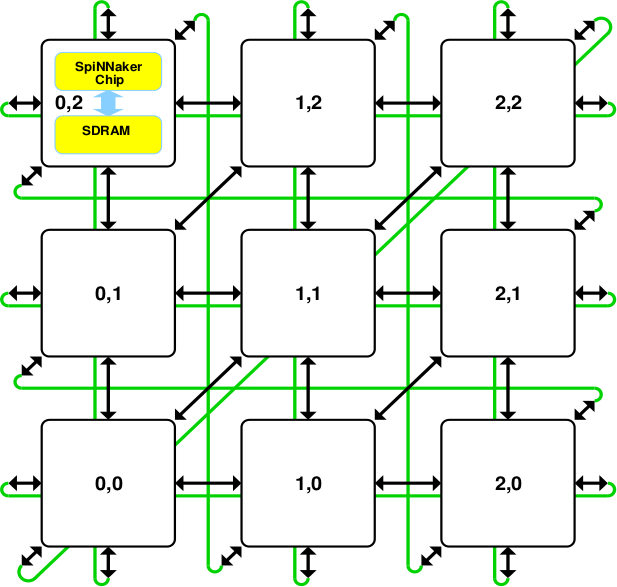
\includegraphics[width=0.5\textwidth]{grid}
\caption{Chip Grid}
\label{fig:grid}
\end{center}
\end{figure}

The important thing to note is that they can communicate between them in a triangle manner (as shown by the arrows).\\

The SpiNNaker provides different mechanisms to communicate between intrachip and interchip cores. In this document only one is discussed. This is the \textbf{multicast messaging}. This type of system enables the user to send messages to one or more nodes, which actually fits the balancer structure needs perfectly.\\

In order to specify the message target, a \textbf{multicast table} has to be filled. This can be seen as a routing table, and there is a distinct one for each chip. Cores within a chip share the same table.\\
Each row is filled in the following way:
\[
[key  -  mask -  target]
\]
The API provides a function for filling the table and a function for sending messages. These are \textit{spin1\_set\_mc\_table\_entry} and \textit{spin1\_send\_mc\_packet}, respectively. Note that in order to fill the table, the user must also specify the row which will contain the entry. This is used as a priority setup, as entries placed at the top of the table will be read before entries later located and will therefore have priority if conflicts are found (e.g., entries sharing the same key).\\

The other important parameters are the \textbf{key}, the \textbf{mask} and the \textbf{target}. The first one is used to specify the message type and can take any value. The mask is used in order to select the key bits relevant for routing. This is analogous to a normal router, as masked bits are not used for selecting the destination and are ignored. In practice, this mechanism is used if more than a core sends a message to the same target. By masking certains key bits, the sending core can add its own identifier, so that the receiving core knows who sent the message.\\
The last parameter specifies the target. Every bit codes for a particular destination. If it is set to 1, then the packet is routed toward a particular location. The format is given by:
\[
[ 0 (11) - core (15) - chip (6)]
\]
Every bit within the \textit{core} range codes for a core situated in the current chip, whereas the \textit{chip} bits specify toward which chip the message should be forwarded. \\
There are to standards to follow. The first concerns the cores:
\begin{verbatim}
....0001.... core 1
....0010.... core 2
....0100.... core 3
....1000.... core 4
... etc...
\end{verbatim}

The second is about the chip destinations (they are consistent with the grid image):
\begin{verbatim}
....000001 EAST
....000010 NORTH EAST
....000100 NORTH
....001000 WEST
....010000 SOUTH WEST
....100000 SOUTH
\end{verbatim}

Finally, a complex example resuming all the mechanism is proposed.\\
Assuming \textit{(core 1; chip 0,0)} wants to send a message toward cores \textit{(core 5; chip 0,0)} and \textit{(core 3; chip 1,1)}. This message has key \textit{0xB00000000} and the rest of the bits are used to send some information to the targets.\\
Then, the multicast tables for the two chips should have such entries:
\begin{verbatim}
// table on chip 0,0
[ 0xB0000000 - 0xF0000000 - (1 << (5 + 6)) | (1 << 1) ]
                                   // core | chip
								
// table on chip 1,1
[ 0xB0000000 - 0xF0000000 - (1 << (3 + 6)) ]
                                   // core
\end{verbatim}


\subsection{Network Communication}
This sub-section details the parallelization strategy adopted to speed-up the algorithm. \\

As stated in the previous sections, the plate is discretized so that each neuron population is located at some point on it and has some receptive field.\\
A good approach toward the parallelization is to place every population on a different core. In addition, a master core would gather all the nodes information and send commands to the motors. Using this strategy, we mimic at 100\% the brain structure, because we would have a population on each core communicating with adjacent populations. The network is composed of a master core located at \textit{(core 1; chip 0,0)}, and 59 slave nodes. Note that on every chip we can actually only use 15 cores and we already use 1 for the master. However, the populations of the 5 missing cores are situated near the plate center, where we have a high population density. Therefore we do not loose much sensitivity on that location.\\
For every algorithm iteration, the protocol for information exchanging  is the following:

\begin{itemize}
\item Master node computes the \textit{error} and the new motor commands.
\item Master node sends new ball position and \textit{error} to all slaves.
\item Slave nodes perform weight updating.
\item Slave nodes send new weights (actually weight*\(\phi(x)\)) to master node.
\end{itemize}

A crucial point is that in order for this stategy to work perfectly, the entire message exchanging phase should take less time than \(\Delta t \), otherwise inconsistencies are introduced. \\

Therefore, optimization is very important in this situation. Indeed, nodes should never send more than one message per iteration, otherwise too much time is spent. The problem is that when using multicast messages, at most only 64 bits of data are available (key + payload). But the master node needs to send 2 floating error values (x and y) and the ball position. Even worse, each slave has to send its own identifier and 4 different floating weights! Even if integer values can be highly optimized, how should one handle floating numbers ?\\
There is however a way to send all this information using only one message on each side. The system takes advantage of the fact that every floating number (error and weights) lies in the range [-1;1]. It is possible to multiply these numbers by a certain value and convert them to integers, so that they can be well packed. During the conversion we loose only a very small fraction of the floating number, therefore not introducing important errors.\\

The two types of messages are the error (\textit{ERROR\_MSG}) and the updating (\textit{UPD\_MSG}).\\

The error is defined by:
\begin{verbatim}
#define ERROR_MSG (uint)(0xA0000000) // mask is 0xF0000000
\end{verbatim}
and its format is (key and payload respectively):
\[
[ A (4) - 0 (10) - sign (2) - x (8) - y (8)] 
\]

\[
[ error_x (16) - error_y (16) ]
\]
Two points are worth noting: the first is that the error is multiplied by 10000 and then transformed into an integer, therefore occupying at most 16 bits. The other point is that in order to deal with negative values, two sign bits are introducted, one for each error.\\

The update message is defined by:
\begin{verbatim}
#define UPD_MSG (uint)(0x40000000) // mask is 0xC0000000
\end{verbatim}
and its format is (key and payload respectively):
\[
[ 4 (2) - sign (4) - index (6) - v_x (10) - v_y (10)]
\]

\[
[\theta (16) - \psi (16)]
\]
The Actor network values are multiplied by 10000 and transformed into integers, as in the previous format. However, the Critic network values are multiplied only by 1000, thus occupying at most 10 bits. Also note that there 4 sign bits as well.


\section{Results}




\section{Conclusion}

\section{Appendix}
\subsection*{A. Constants}
The constant values used in the simulation are provided in this appendix.

\begin{multicols}{2}
\[ 
\Delta t = 0.1 sec
\]

\[
\tau = 0.101
\]

\[
\kappa = 0.101
\]

\[
\gamma = 0.01
\]

\[
\lambda = 1
\]

\[
\eta^{V} = 0.5
\]

\[
\eta^{A} = 0.5
\]

\[
N^{V} = 64
\]


\[
N^{A} = 64
\]

\[
k = 0.5
\]

\[
\sigma_{0} = 0.1
\]

\[
\tau_{m} = 2
\]

\[
\beta = 5
\]

\[ 
\alpha = 0.8
\]
\end{multicols}

\subsection*{B. SpiNNaker API Functions}
In this appendix, the most important API functions are listed.
\begin{verbatim}

/*
Returns the chip and the core 
virtual identifiers of the current node
*/
uint spin1_get_core_id();
uint spin1_get_chip_id();


/*
Prints a message in the tubotron (a visualization tool)
*/
void io_printf(IO_STD, char* msg, params...);


/*
Sets the timer before a TIMER_TICK event is
launched. The value is in microseconds.
*/
void spin1_set_timer_tick(uint TICK_TIME)

	
/*
Creates a callback on an event (MC_PACKET_RECEIVED,
TIMER_TICK, etc...)
*/
void spin1_callback_on(uint EVENT_TYPE, fct(...), uint priority)


/*
Fills a multicast table entry. Returns SUCCESS or FAILURE
*/
uint spin1_set_mc_table_entry(uint row, uint key, uint mask, uint target)


/*
Send a multicast message. Needs to know if the payload is
present or not. Returns SUCCESS or FAILURE
*/
uint spin1_send_mc_packet(uint key, uint pauload, uint p_present)


/*
Starts the simulation on the node
*/
void spin1_start();
\end{verbatim}


\section{References}
\end{document}